\subsection{Wick-Theorem}

\begin{itemize}
  \item Beachte: Erwartungswert ist imernoch im ww-freien Grundzustand
  \item $\psi_0, \psi_0^\dagger$ nur Zeitentwicklung gemäß H 0\\
        $\rightarrow$ Die Berechnung des Erwartungswertes analog zu freien Teilchen
  \item Wick-Theorem: Operator Identität und damit exakt
\end{itemize}

\begin{center}
  \fbox{%
    \begin{minipage}{0.95\linewidth}
      \raggedright
      \setlength{\parindent}{0pt}
      \setlength{\parskip}{0.8\baselineskip}

      Der Erwartungswert eines Produktes einer beliebigen (geraden) Anzahl von Feldoperatoren $\psi_0$ und $\psi_0^\dagger$ in der Wechselwirkungsdarstellung ist gleich der Summe der Produkte aller möglichen paarweise Erwartungswerte (Kontraktionen) dieser Operatoren.

      In jedem Operatorpaar stehen die Operatoren in der gleichen Reihenfolge, wie im ursprünglichen Erwartungswert.

      Das Vorzeichen eines jeden Summanden ist $(-1)^P$, wobei $P$ die Anzahl der notwendigen Vertauschungen ist, um die Operatoren nebeneinander zu bringen.

      Von Null verschieden sind nur die Kontraktionen mit $\psi$ und $\psi^\dagger$. (Im diagonalen Matrixelement müssen Teilchen, die durch $\psi^\dagger$ erzeugt werden, durch $\psi$ wieder vernichtet werden, und umgekehrt.)

      Die Anwendung des Wick-Theorems ergibt Produkte von Erwartungswerten paarweise zeitgeordneter Feldoperatoren $\psi$ und $\psi^\dagger$, also Greensche Funktionen freier Teilchen.

      Siehe auch: StudIP 07\_Wick-Theorem.pdf\\
      G.C. Wick, \textit{Phys. Rev.} 80, 268 (1950)\\
      Fetter and Walecka, \textit{Quantum Theory of Many-Particle Systems}
    \end{minipage}%
  }
\end{center}

Das Wick-Theorem liefert Produkte von zeitgeordneten Erwartungswerten:
\begin{align}
  G^{(0)}(1,1\mkern1mu')
   & = -\frac{i}{\hbar}\,\erw{T\!\left[\psi_0(1)\,\psi_0^\dagger(1\mkern1mu')\right]}
  \quad \text{(freie GF)}
\end{align}
\begin{equation}
  \begin{aligned}
    G^{(1)}(1,2)
     & = \erw{T\!\left[\psi_0(1)\,\psi_0^\dagger(2)\,\psi_0^\dagger(3)\,\psi_0^\dagger(4)\psi_0(4)\,\psi_0(3)\right]}\,V(3-4) \\
     & = (i\hbar)^3\Big\{
    G_0(1,2)\Big[
              \underbrace{G_0(3,3_+)G_0(4,4_+)}_{\textcolor{red}{\text{a)}}}
              -
              \underbrace{G_0(3,4)G_0(4,3)}_{\textcolor{red}{\text{b)}}}
              \Big]                                                   \\
     & \qquad\;
    - G_0(1,3)\Big[
                \underbrace{G_0(4,4_+)G_0(3,2)}_{\textcolor{red}{\text{c)}}}
                -
                \underbrace{G_0(3,4)G_0(4,2)}_{\textcolor{red}{\text{d)}}}
                \Big]                                                   \\
     & \qquad\;
    - G_0(1,4)\Big[
                \underbrace{G_0(3,3_+)G_0(4,2)}_{\textcolor{red}{\text{c)}}}
                -
                \underbrace{G_0(4,3)G_0(3,2)}_{\textcolor{red}{\text{d)}}}
                \Big]
    \Big\}\,V(3-4)\,.
  \end{aligned}
\end{equation}
Folgende Anmerkungen fürs Verständnis:
\begin{itemize}
  \item Variablen 1, 1', 2, 2' wurden hier der Einfachheit halber in 1, 2, 3, 4 umbenannt
  \item Genau genommen sind es keine Gleichungen da $G^{(1)}(1,1\mkern1mu')$ in \autoref{f:entw_G(1,1')} angegebn ist
  \item Der erste Gleichheitsschritt ist somit einfach nur das Anwenden des Wick-Theorems auf die Erwartungswerte von sechs Operatoren
\end{itemize}

\subsubsection*{Feynman-Diagramm}

% --- Kurze Legende für Diagramme ---
\paragraph{Diagramm-Legende}
Jedem Summanden wird ein spezielles Diagramm zugeordnet (Punkte, Linien, Wellenlinien):
\begin{itemize}
  \item Punkt (Variablen-Satz 1 = $r_1,t_1,s_1$) wird einem Punkt zugeordnet: \icon{dot.png}
  \item Durchgezogene Linie is die freie GF: $G_0(1,1\mkern1mu')$ \icon{line.png}\\
        $\rightarrow$ Für gleiche Argumente $G_0(1,1)$: \icon[6ex]{circle.png}
  \item Wellenlinie: Wechselwirkung $V$ \icon[2.2ex]{wave.png}
  \item Über alle inneren Punkte wird integriert (Summen/Integrale an den Symbolen zuordnen)
\end{itemize}
\begin{figure}[ht]
  \centering
  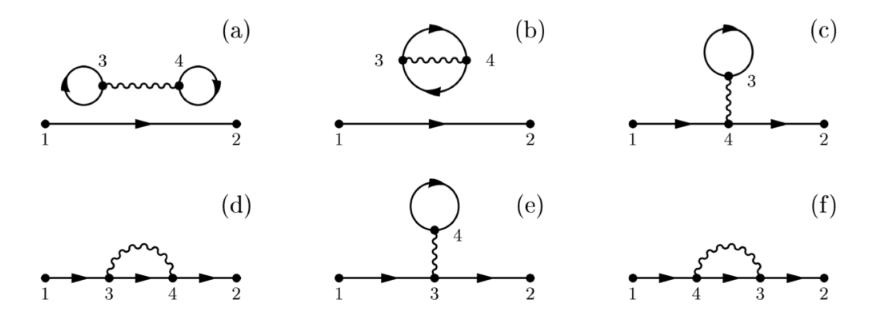
\includegraphics[width=0.8\textwidth]{Pictures/Feynman_for_Coulomb.png}
  \caption{Feynman-Diagramme für die Terme a) bis f) in der Entwicklung von $G^{(1)}(1,2)$.}
  \label{fig:Feynman_Diagramm}
\end{figure}

\lend{Vorl. 04.05.2026}

\subsubsection*{Entwicklung in erster Ordnung der WW}

\begin{itemize}
  \item Zunächst 6 Diagramme
  \item 2 Typen von Diagrammen
        \begin{itemize}
          \item Verbunddiagramme: c--f
          \item Diagramme mit separaten Schleifen: a, b
        \end{itemize}
  \item Unverbundene Anteile entstehen, wenn einige zu $H^{(0)}_{\text{int}}$ gehörende Operatoren untereinander kontrahieren, aber nicht mit $\psi_0(1)\psi_0^\dagger(2)$
  \item Solche Summanden sind in $n$-ter Ordnung gegeben durch:
\end{itemize}

\begin{equation}
  \begin{aligned}
    G^{(n)}(1,2)
     & = \frac{-i}{\hbar}\frac{1}{\erw{S}}\frac{1}{n!}\left(\frac{-i}{\hbar}\right)^n
    \int\!\mathrm{d}\bar{t}_1\cdots\!\int\!\mathrm{d}\bar{t}_m\,
    \erw{T\!\left[\psi_0(1)\,\psi_0^\dagger(2)\,H^{(0)}_{\text{int}}(\bar{t}_1)\cdots H^{(0)}_{\text{int}}(\bar{t}_m)\right]} \\
     & \quad\cdot
    \underbrace{\frac{n!}{m!(n-m)!}}_{\shortstack{Zahl der Möglichkeiten\\die $n$ Operatoren in \\zwei Gruppen aufzuteilen}}
    \int\!\mathrm{d}\bar{t}_{m+1}\cdots\!\int\!\mathrm{d}\bar{t}_n\,
    \erw{T\!\left[H^{(0)}_{\text{int}}(\bar{t}_{m_1+1})\cdots H^{(0)}_{\text{int}}(\bar{t}_n)\right]}
  \end{aligned}
\end{equation}

\begin{itemize}
  \item Zu einem Verbunddiagramm in einer bestimmten Ordnung kommen in den folgenden Ordnungen alle möglichen unverbundenen Anteile hinzu.
        \begin{itemize}
          \item Zu allen Diagrammen in \autoref{fig:Feynman_Diagramm} kommen in zweiter Ordnung die unverbundenen Anteile von a) und b) hinzu.
          \item Theoretisch kann in zweiter Ordnung alle Diagramme aus erster Ordnung mit dem unverbundenen Anteil kombiniert werden der von 1 $\to$ 2 geht.
        \end{itemize}
  \item Zu den Verbunddiagrammen $n$-ter Ordnung addieren sich in den folgenden Ordnungen alle Diagramme, die dieses Verbunddiagramm und zusätzlich unverbundene Anteile enthalten.
\end{itemize}

\begin{equation}
  \begin{aligned}
    G^{(n)}(1,2)
     & = \frac{-i}{\hbar}\frac{1}{\erw{S}}\frac{1}{m!}\left(\frac{-i}{\hbar}\right)^m
    \int\!\mathrm{d}\bar{t}_1\cdots\!\int\!\mathrm{d}\bar{t}_m\,
    \erw{T\!\left[\psi_0(1)\,\psi_0^\dagger(2)\,H^{(0)}_{\text{int}}(\bar{t}_1)\cdots H^{(0)}_{\text{int}}(\bar{t}_m)\right]}   \\
     & \underbrace{\quad\cdot \sum\limits_{n=m}^{\infty}\!
         \frac{1}{(n-m)!} \left(\frac{-i}{\hbar}\right)^{n-m} \int\!\mathrm{d}\bar{t}_{m_1+1}\cdots\!\int\!\mathrm{d}\bar{t}_n\,
         \erw{T\!\left[H^{(0)}_{\text{int}}(\bar{t}_{m_1+1})\cdots H^{(0)}_{\text{int}}(\bar{t}_n)\right]}}_{\erw{S}}
  \end{aligned}
\end{equation}

$\Rightarrow$ In der Störungsreihe der GF kürzt sich der Vorfaktor $\frac{1}{\erw{S}}$ gerade gegen die Beiträge der unverbundenen Diagramme weg\\
$\qquad \hookrightarrow$ Das Kürzen funktioniert nur, wenn man unendlich viele Summanden also Ordnungen hat
\begin{itemize}
  \item Zur weiteren Vereinfachung: Zsf. Von Diagrammen bzw. Summandem, die sich nur in der Bezeichnung unterscheiden
        \begin{itemize}
          \item n-te Ordnung entstehen n Linien der WW \icon[2.5ex]{wave.png}
          \item  n! äquivalente Diagramme durch Permutieren aller n Paar (1,1') $\to$ Vertauschung der Verbindung $\Rightarrow$ 1/n! kürzen
          \item 2$^n$ äquivalente Diagramme durch Vertauschen von 1 und 1' an einer WW $\Rightarrow$ 1/2 kürzen
        \end{itemize}
  \item Bei anderen WW als Coulomb kürzen sich Terme maybe nicht; WW haben im allg. aber nicht mehr als vier Operatoren
\end{itemize}

\subsubsection*{Zusammenfassung der Störungsentwicklung von G(1,2)}

\begin{equation}
  \begin{aligned}
    G(1,2)                                                                      & = G^{(0)}(1,2)                                 & \qquad \text{0.Ordnung} \\
                                                                                & + i\hbar\int\!\mathrm{d}3\!\int\!\mathrm{d}4\,
    \left[ G_0(1,3)G_0(3,4)G_0(4,2) - G_0(1,3)G_0(4,4)G_0(4,2) \right]   V(3-4) & \qquad \text{1.Ordnung}                                                  \\
  \end{aligned}
\end{equation}

\begin{figure}[ht]
  \centering
  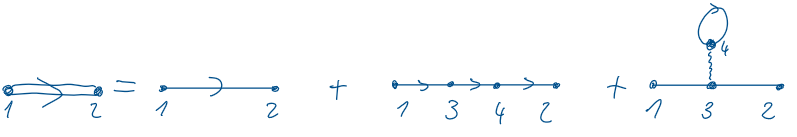
\includegraphics[width=0.8\textwidth]{Pictures/chem_feynman_1Ordnung.png}
  \caption{Chematische Darstellung der Feynman-Diagramme für die Störungsentwicklung von $G(1,2)$ bis zur ersten Ordnung. Alle doppelten bzw. unnötigen wurden direkt rausgekürzt. Dadurch Fallen die Terme $1/n!$ und $1/2$ weg. Allgemein ist mit der Wellenlinie immer $i\hbar V$ gemeint. Deswegen fehlt der Term in dem Bild.}
  \label{fig:chem_feynman_1ord}
\end{figure}

\lend{Vorl. 08.05.2026 }